\begin{figure}[t]
\centering
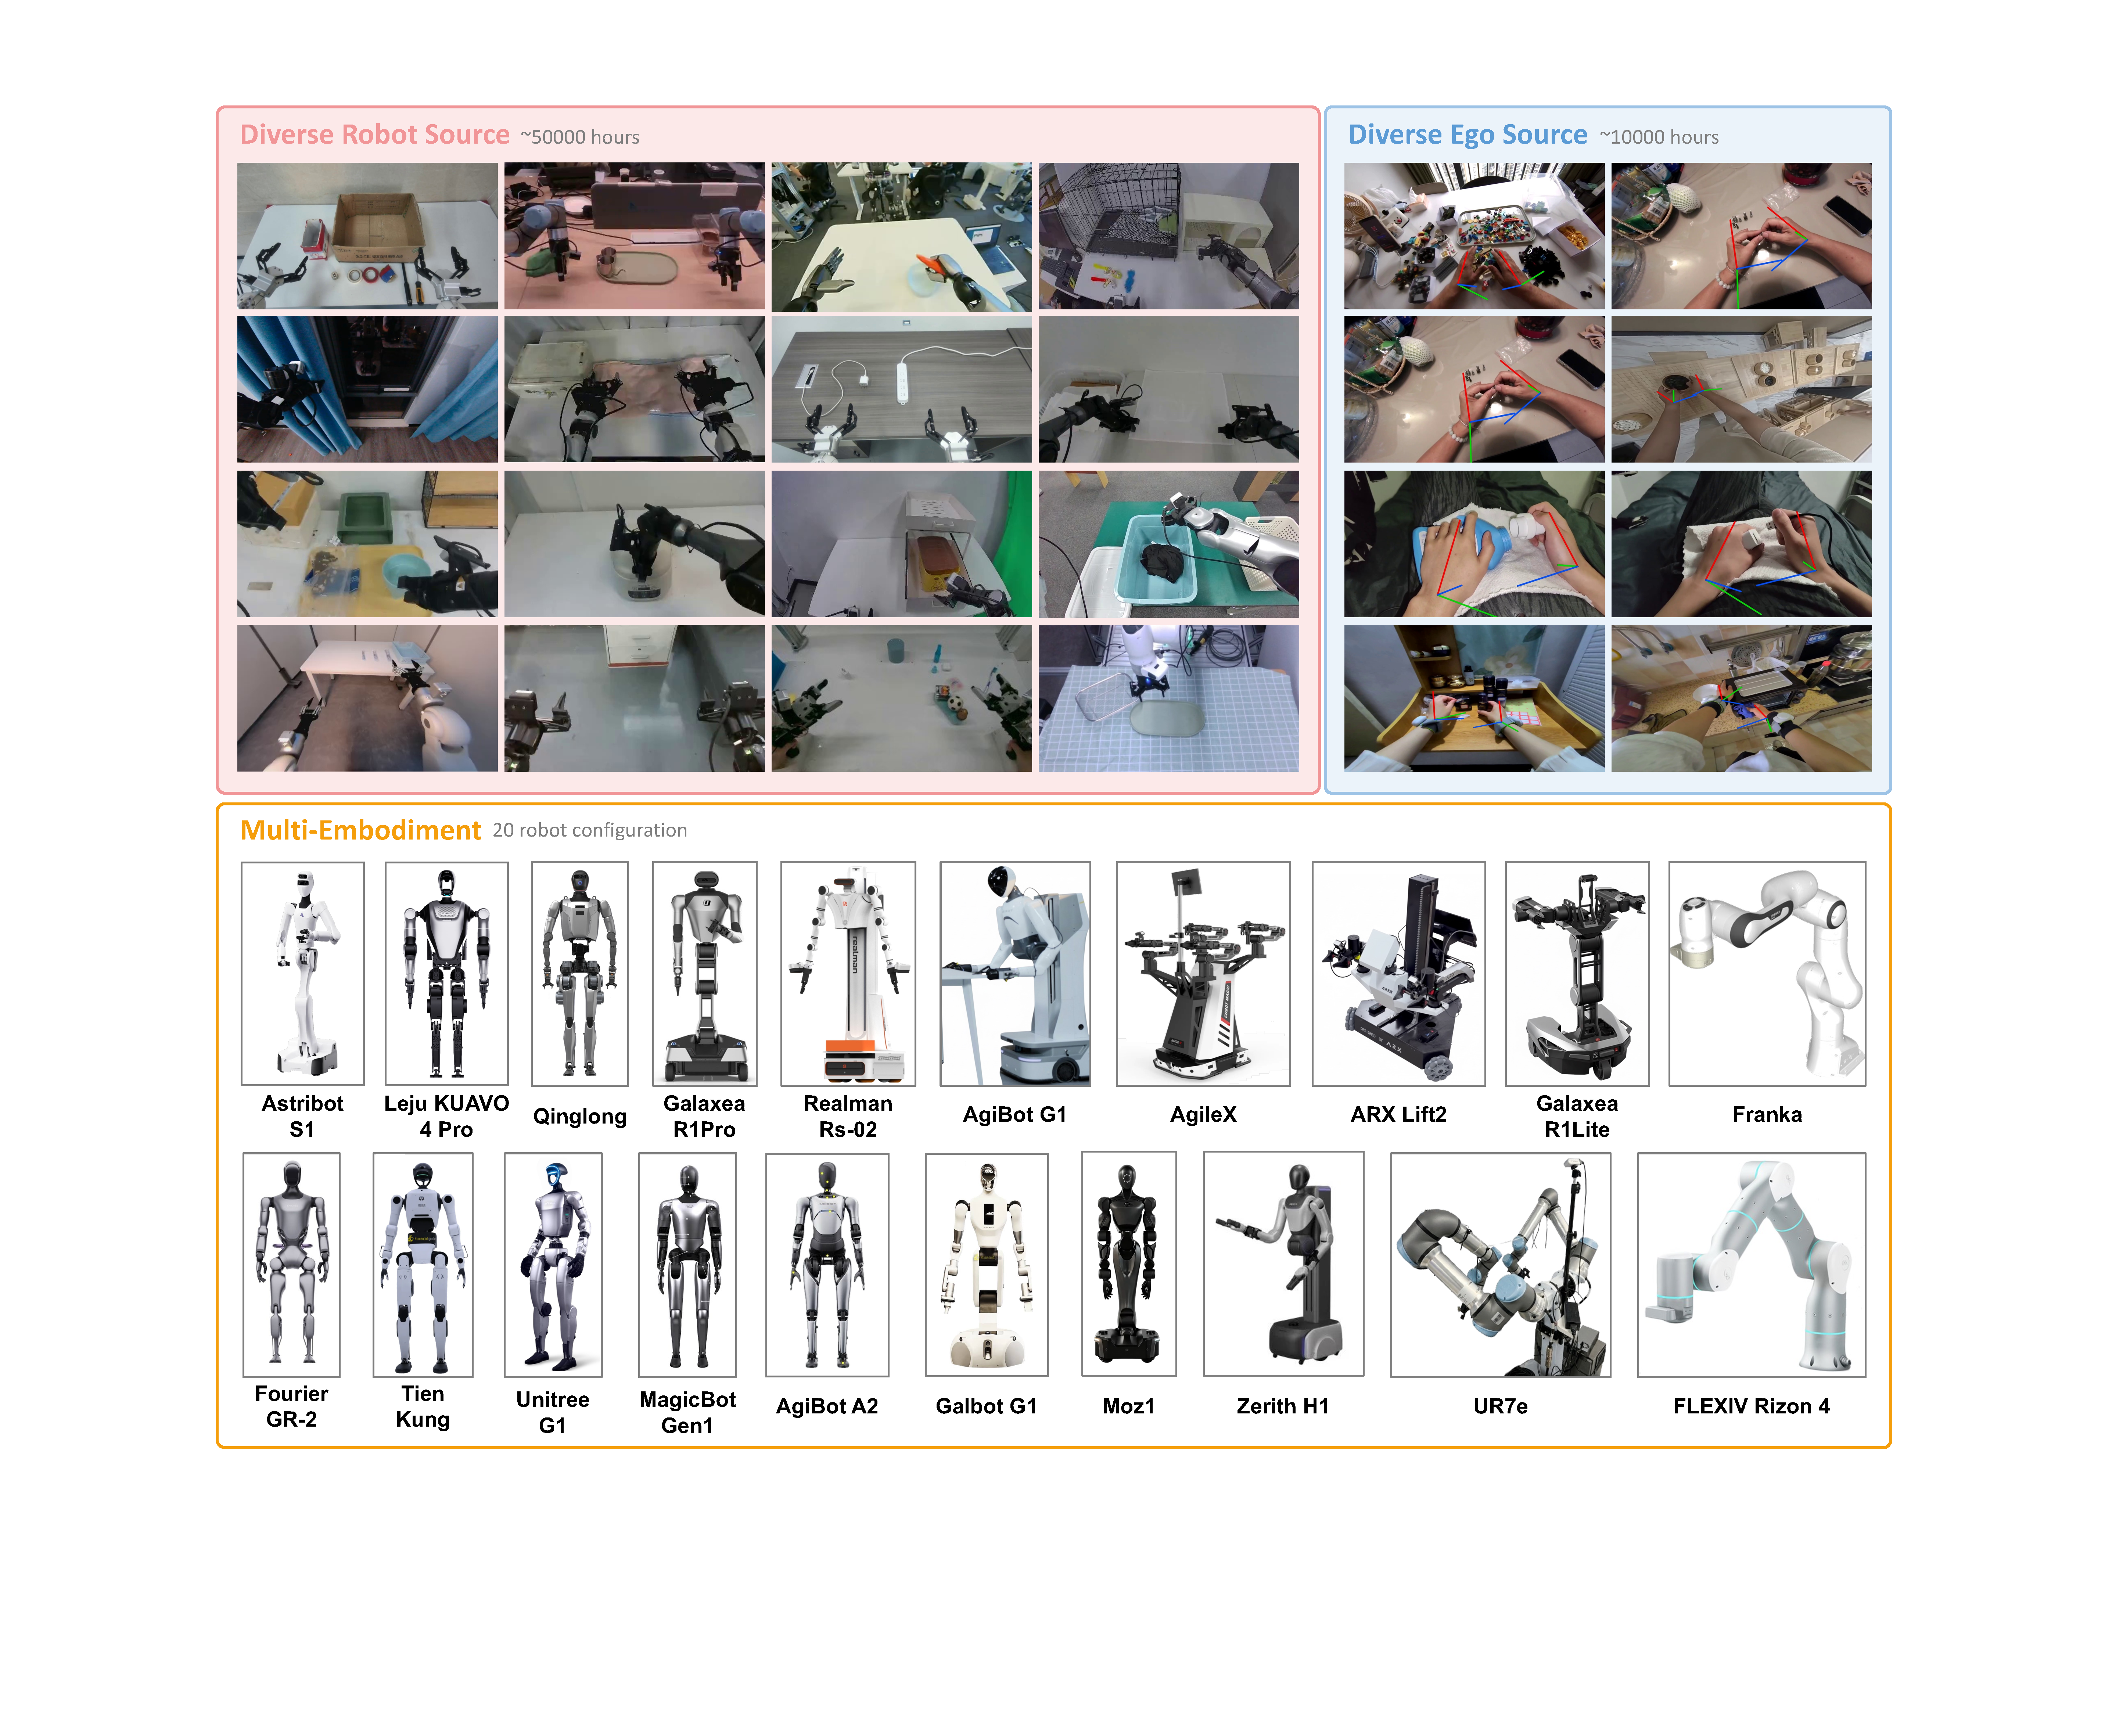
\includegraphics[width=\linewidth]{figures/data_demo.pdf}
\caption{\textbf{Visualization of the pre-training dataset used by LingBot-VLA-2.0}. The dataset includes 20 robot embodiments with degrees of freedom in the arms, heads, waists, mobile bases, and dexterous hands.}
\label{fig:data_demo}
\end{figure}

\section{Related Work}\label{sec:related}


\subsection{Generalist Robot Manipulation Policies}
Recent vision-language-action (VLA) models~\cite{pi_0, pi_0d5, gr00tN1, gr00t_n1_6, gemini_robotics, walloss, galaxeaG0, magma, gr3,abotm0,abotm05,hyembodied05x,qwenrobotmanip,qwenVLA,cai2026xiaomi} have established foundation VLA model as a promising paradigm for generalist robot control. Existing efforts have improved VLA systems along several complementary directions, including scaling heterogeneous robot data and unified pretraining recipes for generalization across tasks and embodiments~\cite{qwenVLA,walloss,wallOSS05,starVLAalpha}, leveraging human-centric data such as egocentric videos and hand motion to learn transferable embodied priors~\cite{beingH0,beingH05,beingH07}, introducing embodiment-aware architectures or unified action spaces to better support cross-platform transfer~\cite{holoBrain0}, and incorporating predictive or world-modeling objectives to improve temporal reasoning and future-aware decision making~\cite{lda1b,dexWorldModel}. Other works further enhance VLA models through geometry-aware supervision~\cite{gem}, autoregressive reasoning-action unification~\cite{g0_5}, or deployment-oriented system design for real-world execution~\cite{rldx1,walloss}. Together, these studies demonstrate the rapid progress of foundation VLA models, while also highlighting that practical deployment still requires jointly addressing large-scale generalization, richer embodiment, and action-space support.

\subsection{Mixture-of-Experts Vision-Language-Action Model}
Mixture-of-Experts (MoE) has emerged as a pivotal mechanism for scaling action modeling capacity in VLA systems.
For contact-rich manipulation, ForceVLA~\cite{forcevla} and ForceVLA2~\cite{forcevla2} introduce force-aware MoE modules to fuse sparse but critical force feedback with visual-language representations, while MoDE-VLA~\cite{modevla} further exploits force and tactile signals for dexterous bimanual manipulation. 
For long-horizon tasks, AtomicVLA~\cite{atomicvla} structures experts around atomic skills to mitigate inter-stage interference, while SAMoE-VLA~\cite{samoevla} conditions expert routing on scene-level representations rather than token-level features alone.
Other works~\cite{hex,himoevla, beingH05} introduce MoE structures to address humanoid body-part and motion-phase specialization, and embodiment-level heterogeneity.
In large-scale VLA pretraining, action representations are jointly shaped by multiple entangled factors, including embodiment-specific dynamics, task-dependent control logic, and deployment scenario diversity. Rather than prescribing expert semantics based on any single dimension of variation, we instantiate token-level sparse MoE layers within the action expert, enabling each action token to adaptively select experts based on its intrinsic features. Furthermore, we adopt an auxiliary-loss-free load-balancing mechanism~\cite{liu2024deepseek} that promotes balanced expert utilization via routing correction biases, eliminating the need to inject an explicit load-balancing loss into the primary action learning objective.












